\documentclass[11pt,a4paper]{article}
\usepackage{amsmath,amssymb,graphicx,geometry,booktabs,hyperref,longtable}
\usepackage{setspace}
\usepackage{siunitx}
\usepackage{placeins}
\onehalfspacing
\emergencystretch=3em
\geometry{margin=1in}

\title{\textbf{IFRS~9 Hedge Accounting for a Quanto Knock-Out Structure}}
\author{\textbf{Jihong Park} \\ Pusan National University}
\date{July 2026}

\begin{document}

\maketitle

\begin{abstract}
A Korean crude-oil importer's commodity-and-currency exposure can be hedged under IFRS~9 either as one combined instrument (a quanto knock-out call) or as two independent risk-component designations. This paper builds a full path-wise cash-flow-hedge accounting engine to quantify how the two architectures differ on hedge ineffectiveness, OCI dynamics, and the economic risk surviving a knock-out event. The combined designation's mean ineffectiveness comes out roughly three-and-a-half times larger than the split designation's, almost entirely from the split structure's commodity leg rather than its currency leg, while full-horizon economic risk is statistically indistinguishable between the two. Extending the comparison to barrier-free variants of both designations isolates the driver: the split leg's ineffectiveness collapses to a mechanically exact zero regardless of the barrier, while the combined structure's stays an order of magnitude larger in every configuration tested, so what drives its elevated ineffectiveness is multiplying two floating exposures into one payoff, not the knock-out feature itself. Every headline figure is traced directly to the accounting engine's own live computation, and a verified accounting identity (the derivative asset equals the OCI reserve plus retained earnings exactly, at every step) confirms the engine's integrity independently of the pricing layer.
\end{abstract}

\tableofcontents
\newpage

% =============================================================================
\section{Introduction}
\label{sec:intro}

A Korean crude-oil importer with a fixed monthly physical requirement of barrels$=2{,}000{,}000$ (equivalently a USD funding need of roughly \$157.88 million per month at inception) is exposed to two risk factors that enter the KRW cost of imported crude \emph{multiplicatively}: the US-dollar price of WTI, $S_1$, and the USD/KRW exchange rate, $S_2$. Neither risk factor alone determines the cash outflow; the product $S_1\cdot S_2$ does. IFRS~9 explicitly recognizes this kind of joint exposure under the heading of an \emph{aggregated exposure} (IFRS~9.6.3.4): a combination of a commodity price risk component and a foreign-currency risk component that together create a single, differently-shaped exposure, which may itself be designated as the hedged item in a cash-flow hedge.

That single aggregated-exposure framing admits two structurally different accounting architectures, and this paper's entire empirical exercise is to measure, not assume, how they differ:

\begin{itemize}
\item \textbf{Structure~A} designates a single hedging instrument, a double knock-out (KO) quanto call whose payoff already multiplies the WTI intrinsic value by the floating terminal FX rate, against the aggregated exposure as a whole. One hedging instrument, one hedge relationship.
\item \textbf{Structure~B} instead exercises IFRS~9's separate permission (9.6.3.1) to designate hedges against individually identifiable and reliably measurable risk \emph{components}: a WTI KO call priced with FX held fixed at inception (isolating pure commodity-price risk), paired with an independent Garman--Kohlhagen FX call on a notional fixed at inception (isolating pure currency risk). Two hedging instruments, two hedge relationships.
\end{itemize}

The distinction is not cosmetic. It is visible directly in the payoff formulas (Section~\ref{sec:arch}): Structure~A's payoff multiplies by the \emph{floating} $S_2(T)$, creating a genuine quanto correlation coupling between the two risk factors inside a single instrument; Structure~B's WTI leg multiplies by the \emph{fixed} $S_2(0)$, deliberately severing that coupling so that the leg prices and hedges commodity risk alone. This paper builds both architectures on an identical, jointly-simulated correlated jump-diffusion path bank, applies the full IFRS~9 cash-flow-hedge accounting mechanics (hypothetical-derivative lower-of testing, cost-of-hedging amortization, knock-out discontinuation, OCI reclassification) to each path at daily granularity, and reports the resulting statement-of-financial-position (SFP), other-comprehensive-income (OCI), ineffectiveness, and economic-residual metrics as measured outcomes.

The underlying quanto KO product (its jump-diffusion dynamics, its Longstaff--Schwartz regression pricing surface, and its double-barrier touch mechanics) is specified fully in Section~\ref{sec:product} of this paper; this paper's entire contribution is on top of that pricing layer, in the accounting-designation question, and Section~\ref{sec:product} is written to be self-contained.

The remainder of the paper proceeds as follows. Section~\ref{sec:litreview} places the model in the IFRS~9 and quanto-pricing literature. Section~\ref{sec:product} derives the underlying jump-diffusion dynamics, the quanto payoff construction, the double-barrier touch probabilities, and the Longstaff--Schwartz pricing algorithm from first principles. Section~\ref{sec:arch} specifies the two designation architectures precisely. Section~\ref{sec:hd} derives the hypothetical derivative that makes Structure~A's effectiveness test non-tautological. Section~\ref{sec:engine} specifies the full accounting engine, including its numerical safeguards and the exact per-step processing sequence. Section~\ref{sec:econ} defines the economic-residual layer. Section~\ref{sec:results} reports measured results. Section~\ref{sec:sensitivity} and Section~\ref{sec:discussion} discuss sensitivities and the central trade-off. Section~\ref{sec:limitations} outlines the model boundaries, and Section~\ref{sec:conclusion} concludes.

% =============================================================================
\section{Literature Review}
\label{sec:litreview}

IFRS~9 (IASB, 2014) requires cash-flow-hedge accounting to recognize the effective portion of a hedging instrument's fair-value change in other comprehensive income, with any ineffective portion in profit or loss, determined by a lower-of test between the cumulative change in the hedging instrument and the cumulative change in a hypothetical derivative representing the hedged item (IFRS~9.B6.5.5, 9.6.5.11). Aggregated exposures (combinations of a non-derivative exposure and a derivative, or of two risk components managed together) may be designated as a single hedged item under 9.6.3.4; risk components of that same exposure may alternatively be hedged individually under 9.6.3.1, provided each component is separately identifiable and reliably measurable. For option-based hedging instruments, IFRS~9 permits the time-value component to be accounted for as a cost of hedging, amortized to profit or loss on a systematic basis separate from the intrinsic-value-based lower-of test (9.6.5.15--9.6.5.16). On discontinuation of a hedge relationship (including when the hedged forecast transaction is no longer expected to occur, or here, when a knock-out event extinguishes the hedging instrument), amounts accumulated in OCI are addressed under 9.6.5.11(d)/9.6.5.12. This paper implements these mechanics path-by-path at daily granularity rather than asserting their qualitative consequences from first principles.

The pricing side draws on three classical results. Merton (1976) supplies the jump-diffusion framework used for WTI, in which discontinuous jump risk renders the market incomplete and a diversifiable jump-risk premium survives the risk-neutral measure change. Longstaff and Schwartz (2001) supply the least-squares Monte Carlo regression used to price and differentiate the barrier-and-early-exercise-aware WTI surface. Garman and Kohlhagen (1983) supply the closed-form currency option formula used for Structure~B's FX leg, which has no barrier feature and therefore needs no regression. Black (1976) supplies the forward-based commodity option convention underlying the WTI premium quoting convention used throughout. The double-KO barrier's discrete-monitoring treatment follows the continuity correction of Broadie, Glasserman, and Kou (1997), applied on the same daily path bank that determines every accounting statistic reported below, so that the same discretization choice that fixes the option's price also fixes its ineffectiveness. The quanto correlation coupling between $S_1$ and $S_2$ inside Structure~A's single-instrument payoff, the kind of coupling Reiner (1992) prices in closed form for a continuously-monitored, barrier-free quanto claim, is handled here instead by joint Monte Carlo simulation of the correlated pair, since no closed form of that kind survives the addition of a discretely monitored double barrier; the design choice is justified formally in Section~\ref{sec:product}.

Why a firm designates a hedge relationship at all (accepting the documentation burden, the effectiveness testing, and the cost-of-hedging amortization mechanics of IFRS~9, rather than simply booking the derivative at fair value through profit or loss) is a question this paper's engine answers quantitatively (by measuring what hedge accounting changes about the P\&L path) but does not itself motivate theoretically. That motivation belongs to the corporate hedging literature: Froot, Scharfstein, and Stein (1993) model hedging as a device for protecting a firm's internal financing capacity, which is the same underlying economic motive that hedge accounting's smoothing of OCI volatility is designed to make visible in the financial statements rather than obscure it; Stulz (1996) develops the practitioner corollary that partial, selective hedging can be value-preserving even when full economic coverage is affordable, directly relevant to Structure~B's asymmetric ineffectiveness split between its WTI and FX legs (Section~\ref{sec:h1}). On the accounting-choice question specifically (whether the designation architecture itself, not just the hedge, is shaped by accounting rather than purely economic considerations), Glaum and Kl\"ocker (2011) document that hedge-accounting eligibility rules measurably influence which economic hedges firms actually put on, a finding this paper's own result (two economically similar architectures producing materially different recognized ineffectiveness) is a quantitative, instrument-level instance of.

% =============================================================================
\section{Product and Pricing Definition}
\label{sec:product}

This section specifies, completely and from first principles, the quanto double-knock-out product whose designation is the subject of this paper. Every accounting formula in Sections~\ref{sec:arch}--\ref{sec:econ} is a function of the objects defined here.

\subsection{Correlated jump-diffusion dynamics}
\label{sec:sde}

Let $S_1(t)$ denote the WTI crude price in USD/bbl and $S_2(t)$ the USD/KRW exchange rate, both evolving under the physical measure $\mathbb P$. $S_1$ is a jump-diffusion process; $S_2$ is a correlated geometric Brownian motion:
\begin{align}
\frac{dS_1(t)}{S_1(t^-)} &= \big(\mu_1^{\mathbb P}-\lambda\kappa\big)dt + \sigma_1\,dW_1(t) + d\!\left(\sum_{j=1}^{N(t)}(e^{Y_j}-1)\right) \\
\frac{dS_2(t)}{S_2(t)} &= \mu_2^{\mathbb P}\,dt + \sigma_2\,dW_2(t) \\
dW_1(t)\cdot dW_2(t) &= \rho\,dt, \qquad \kappa = \mathbb E[e^Y-1] = \exp\!\big(\theta_J+\tfrac12\delta_J^2\big)-1
\end{align}
with $N(t)$ a Poisson process of intensity $\lambda$ and log-jump-sizes $Y_j \overset{\text{iid}}{\sim}\mathcal N(\theta_J,\delta_J^2)$. The production calibration fits $\lambda=6.7846$ jumps per year, $\theta_J=-0.0299$, $\delta_J=0.0844$, a diffusive WTI volatility $\sigma_1=0.3242$, an FX volatility $\sigma_2=0.0926$, and a WTI--FX correlation $\rho=0.0876$.

For simulation under the risk-neutral measure $\mathbb Q$ used for pricing (drift $\mu_1^{\mathbb P}\to r_{US}$, $\mu_2^{\mathbb P}\to r_{KRW}-r_{US}$), the one-step Euler--Maruyama update with the compound Poisson jump superimposed once per step is
\begin{align}
\varepsilon_1 &\sim\mathcal N(0,1), \qquad \varepsilon_2^{\perp}\sim\mathcal N(0,1), \qquad \varepsilon_2 = \rho\varepsilon_1+\sqrt{1-\rho^2}\,\varepsilon_2^{\perp} \\
N_i &\sim\mathrm{Poisson}(\lambda\Delta t), \qquad J_i = \sum_{j=1}^{N_i}Y_j \\
S_1(t_{i+1}) &= S_1(t_i)\exp\!\left[\Big(r_{US}-\lambda\kappa-\tfrac12\sigma_1^2\Big)\Delta t+\sigma_1\sqrt{\Delta t}\,\varepsilon_1+J_i\right] \\
S_2(t_{i+1}) &= S_2(t_i)\exp\!\left[\Big(r_{KRW}-r_{US}-\tfrac12\sigma_2^2\Big)\Delta t+\sigma_2\sqrt{\Delta t}\,\varepsilon_2\right]
\end{align}
The shared shock $\varepsilon_1$ drives both legs' correlated component; this is the same joint construction that Section~\ref{sec:quanto} shows is sufficient, on its own, to price a correlation-coupled quanto payoff without a separate closed-form adjustment.

\subsection{Double knock-out barrier}
\label{sec:barrier}

The structure is monitored against an upper barrier $U=120$ and lower barrier $L=50$ USD/bbl. Let $\tau_{KO}=\inf\{t: S_1(t)\ge U \text{ or } S_1(t)\le L\}$. Because the simulation records $S_1$ only at discrete steps, a path can cross a barrier between two recorded observations without either recorded value lying outside $[L,U]$. The correction applied between each pair of consecutive recorded, interior values $S_1^{\mathrm{prev}},S_1$ is the exact continuous-Brownian-motion conditional touch probability, in log-space:
\begin{align}
p_{up} &= \exp\!\left(\frac{-2\ln(U/S_1^{\mathrm{prev}})\ln(U/S_1)}{\sigma_1^2\Delta t}\right) \\
p_{dn} &= \exp\!\left(\frac{-2\ln(S_1^{\mathrm{prev}}/L)\ln(S_1/L)}{\sigma_1^2\Delta t}\right)
\end{align}
Each is compared against an independent uniform draw once per step; a touch is registered if the draw falls below the corresponding probability. Both formulas are exact under continuous Brownian motion between the two endpoints; a genuine Poisson jump landing strictly between two recorded steps can, in principle, cross a barrier without being captured by either the recorded values or the bridge formula. Formally, the true step-conditional touch probability is
\begin{equation}
\label{eq:jumpgap}
\mathbb P\big(\tau_{KO}\in(t_i,t_{i+1}]\ \big|\ S_1(t_i),S_1(t_{i+1})\big) = p_{up} + \mathcal E_{\mathrm{jump}}(\lambda,\theta_J,\delta_J;\Delta t),
\end{equation}
where $\mathcal E_{\mathrm{jump}}\ge0$ collects paths a jump crosses the barrier on and then reverts into $[L,U]$ by $t_{i+1}$, indistinguishable from a jump-free interior path given only the two recorded endpoints. Since such a path needs both a jump landing within an interval of length $\Delta t$ ($O(\lambda\Delta t)$) and that jump clearing a barrier several diffusive standard deviations away, $\mathcal E_{\mathrm{jump}}=O(\Delta t)\to0$ as $\Delta t\to0$, a small residual gap-risk understatement of the true continuous-time KO frequency. Its size is measured, not merely bounded: a jump-adapted exact re-simulation at $200{,}000$ paths (Poisson jump times drawn exactly within each step, per-sub-interval bridge tests, barrier checked at every jump instant, with the production-style whole-step test evaluated on the \emph{same} paths) puts $\mathcal E_{\mathrm{jump}}$ at $+0.14$ to $+0.18$ percentage points of KO frequency at this daily grid (risk-neutral and physical banks respectively), confirming the $O(\Delta t)$ analysis with a number (Section~\ref{sec:limitations}).

\subsection{Quanto payoff construction and the correlation coupling}
\label{sec:quanto}

The importer's exposure is to the KRW cost of barrels, $\mathrm{barrels}\cdot S_1(t)\,S_2(t)$: both legs enter multiplicatively. The three payoff variants relevant to this paper are (Structure~A's, and the two legs of Structure~B's, are given fully in Section~\ref{sec:arch}); what all of them share is that Structure~A's payoff multiplies the WTI intrinsic value by the \emph{floating} terminal rate $S_2(T)$, so that
\begin{align}
\mathbb E^{\mathbb Q}\!\big[\max(S_1(T)-K,0)\cdot S_2(T)\big] \;\ne\; \mathbb E^{\mathbb Q}\!\big[\max(S_1(T)-K,0)\big]\cdot\mathbb E^{\mathbb Q}\!\big[S_2(T)\big]
\end{align}
whenever $\rho\ne 0$. A closed-form treatment of this coupling ordinarily requires an explicit quanto drift adjustment (a numeraire change that shifts $S_1$'s effective risk-neutral drift by $-\rho\sigma_1\sigma_2$). This engine never writes that adjustment down explicitly: because $S_1$ and $S_2$ are simulated jointly from the correlated shocks of Section~\ref{sec:sde}, every path already carries the true correlated joint realization of $(S_1(T),S_2(T))$, and multiplying the two legs together path-by-path before averaging across paths reproduces the correlation-coupled expectation to simulation accuracy automatically. This is why Structure~B's WTI leg, by contrast, multiplies by the \emph{fixed} $S_2(0)$ rather than $S_2(T)$: fixing the FX conversion rate at inception deliberately removes the quanto coupling from that leg, so that it is a genuine single-risk-factor commodity hedge, mathematically as well as by designation intent. This payoff-level distinction (floating conversion in Structure~A versus fixed conversion in Structure~B's WTI leg) is the precise mathematical counterpart of the IFRS~9 aggregated-exposure-versus-risk-component choice discussed in Section~\ref{sec:arch}.

\subsection{Longstaff--Schwartz pricing surface and backward-induction algorithm}
\label{sec:lsmc}

The engine prices and differentiates the barrier option by least-squares Monte Carlo. Writing $K$ for the strike ($K=S_1(0)$, at-the-money-forward) and normalizing $v_1=S_1/K$, $v_2=S_2/S_2(0)$, the continuation-value surface at each step is a 5-term polynomial,
\begin{equation}
\tilde C(S_1,S_2) = \beta_0+\beta_1v_1+\beta_2v_2+\beta_3v_1^2+\beta_4v_2^2+\beta_5v_1v_2,
\end{equation}
fitted by ordinary least squares on in-the-money, not-yet-knocked-out paths, independently at every discrete step. The procedure: (1) simulate $N$ joint paths forward from $t_0$ to $t_n=T$, recording the first barrier-hitting step via Section~\ref{sec:barrier}'s bridge test; (2) initialize terminal value at $t_n$ from the payoff; (3) step backward from $i=n-1$ to $1$, regressing the one-step-discounted future value on $(v_1,v_2)$ over the surviving in-the-money subset to obtain $\beta_0(t_i),\ldots,\beta_5(t_i)$, and carrying non-fitted paths' discounted future value backward unchanged; (4) average the step-0 cash flows for the price, retaining every step's $\beta$ coefficients as the pricing and hedging surface. Structure~A's option surface and Structure~B's WTI-only surface (fixed-$S_2(0)$ payoff) are fitted \emph{separately}, since their payoffs differ; Structure~B's FX leg needs no regression surface at all, since the Garman--Kohlhagen closed form applies directly to a barrier-free option.

% =============================================================================
\section{Designation Architectures}
\label{sec:arch}

\subsection{Structure A -- single quanto KO designation}
\label{sec:structA}

The hedging instrument is a single European-style quanto KO call. Payoff at maturity, conditional on no knock-out:
\begin{equation}
V_A(T) = \mathrm{barrels}\cdot\max(S_1(T)-K,0)\cdot S_2(T)\cdot\mathbf 1\{\tau_{KO}>T\}, \qquad K=S_1(0).
\end{equation}
Fair value along a path is $\max(\tilde C(S_1,S_2)\cdot\mathrm{barrels},\,\mathrm{intrinsic})$ from Structure~A's own regression surface; the floor at intrinsic value is a no-arbitrage safeguard described in Section~\ref{sec:safeguards}. On knock-out, $V_A\to 0$; the CFH reserve freezes and any unamortized time value is swept to ineffectiveness (Section~\ref{sec:ko}).

\subsection{Structure B -- dual independent designations}
\label{sec:structB}

\paragraph{B1 (WTI KO call).} Payoff $\mathrm{barrels}\cdot\max(S_1(T)-K,0)\cdot S_2(0)\cdot\mathbf 1\{\tau_{KO}>T\}$, priced from a separately-fitted WTI-only regression surface. On knock-out, B1's fair value goes to zero and its remaining time value is swept to ineffectiveness:
\begin{equation}
\text{residual\_TV}_W = \max(\mathrm{TV}_{W,0}-\mathrm{COH}^{\mathrm{amort}}_w,\,0),
\end{equation}
using $\mathrm{TV}_{W,0}$, the \emph{inception} time value (initial fair value minus initial intrinsic), not the already-zeroed post-KO fair value.

\paragraph{B2 (Garman--Kohlhagen FX call).} Strike $G_0=S_2(0)e^{(r_{KRW}-r_{US})T_{FX}}$, notional $N_{FX}=\mathrm{barrels}\cdot F_0^{WTI}$ fixed at inception, while the economically relevant dollar exposure $\mathrm{barrels}\cdot S_1(t)$ is stochastic: a deliberate, fixed-notional structural mismatch. Fair value follows the closed-form Garman--Kohlhagen call,
\begin{equation}
V_{B2}(t) = \mathrm{GKCall}\big(S_2,\,G_0,\,\sigma_2,\,\tau,\,r_{US},\,r_{KRW},\,N_{FX}\big),
\end{equation}
since the leg carries no barrier and needs no regression surface. B2 survives WTI knock-out; its subsequent fair-value changes flow to FVTPL, not OCI (Section~\ref{sec:ko}).

Both B1 and B2 use intrinsic-value-based lower-of comparisons, not a mix of intrinsic value on one side and full fair value (including time value) on the other, which would otherwise bias the two legs' measured effectiveness against each other for reasons unrelated to the underlying hedge quality.

% =============================================================================
\section{The Hypothetical Derivative}
\label{sec:hd}

IFRS~9's lower-of test compares the cumulative change in the hedging instrument against the cumulative change in a hypothetical derivative (HD) that mirrors the hedged risk without hedge-specific features (IFRS~9.B6.5.5). Using Structure~A's own fair value as its HD would make the comparison tautological: $\Delta V_A$ against itself is identically equal, so ineffectiveness would be zero by construction on every path, including knocked-out ones. The hedged item here is a highly probable purchase that does \emph{not} itself knock out; the correct HD is therefore the barrier-free quanto forward on the physical exposure,
\begin{equation}
\label{eq:hstar}
H^\star(t) = \mathrm{barrels}\cdot S_1(t)\,S_2(t)\,\exp\big(\rho\sigma_1\sigma_2(T-t)\big),
\end{equation}
the closed-form risk-neutral expectation of undiscounted physical settlement at $T$, projected from $t$. Because $V_A$ carries the KO indicator and $H^\star$ does not, $\Delta V_A$ and $h_t\Delta H^\star$ (Section~\ref{sec:ht}) are not related by construction: on knocked-out paths $V_A\to 0$ while $H^\star$ continues to track $\mathrm{Phys}(t)=\mathrm{barrels}\cdot S_1(t)S_2(t)$, and cumulative ineffectiveness $\Delta V_A-\Delta\mathrm{CFHR}_A$ can be, and empirically is, materially nonzero.

% =============================================================================
\section{Accounting Engine}
\label{sec:engine}

\subsection{Signed lower-of test}
\label{sec:lowerof}

At each step,
\begin{equation}
\mathrm{SignedLowerOf}(x,y) = \begin{cases} 0 & \text{if } \mathrm{sign}(x)\ne\mathrm{sign}(y) \text{ and both nonzero} \\ \mathrm{sign}(x)\cdot\min(|x|,|y|) & \text{otherwise.} \end{cases}
\end{equation}
The sign-consistency branch is not incidental: if the hedging instrument and the hypothetical derivative (or hedged item) have moved in \emph{opposite} directions since inception, the qualifying economic relationship that the hedge relies on has itself broken down for that comparison, and no positive effective portion should be recognized. Structure~A applies this to $(\Delta V_A-V_{A,0},\ h_t\Delta H^\star)$; Structure~B applies it separately to B1 (intrinsic WTI change versus $\mathrm{barrels}\cdot(S_1-S_1(0))S_2(0)$) and B2 (intrinsic FX change versus intrinsic value evaluated on the floating notional $\mathrm{barrels}\cdot S_1\,e^{r_{US}\tau}$).

\subsection{Cost-of-hedging amortization}
\label{sec:coh}

Inception time value $\mathrm{TV}_0=V_0-\mathrm{Intr}_0$ amortizes straight-line over the horizon, $\mathrm{COH\_step}=\mathrm{TV}_0/\text{steps}$. Remaining deferred time value $\max(\mathrm{TV}-\mathrm{COH}^{\mathrm{amort}},0)$ sits in OCI alongside the CFH reserve until amortized or swept on discontinuation.

\subsection{Knock-out event processing}
\label{sec:ko}

On the KO step, Structure~A sets $V_A=0$, sweeps remaining time value per Section~\ref{sec:structA}, and freezes CFHR/OCI at their KO-moment values. Structure~B zeros B1 and applies its own residual-time-value sweep; B2's COH freezes at its KO-moment leftover ($\max((\mathrm{FV}_x-\mathrm{Intr}_x)-\mathrm{COH}^{\mathrm{amort}}_x,0)$, since B2 economically survives) while its subsequent fair-value changes accrue to $\mathrm{FVTPL}_B$ rather than OCI. This routes \emph{both} legs' post-event treatment off a single shared discontinuation flag triggered by the WTI barrier; Section~\ref{sec:limitations} discusses the tension this creates with Section~\ref{sec:arch}'s framing of B1 and B2 as independent hedge relationships.

\subsection{Dynamic hedge ratio and non-circularity}
\label{sec:ht}

Structure~A's hedge ratio $h_t$ is not backed out by dividing $V_A$ by $H^\star$; it is the analytic sensitivity of the fitted regression surface itself. At step $stp$, with $v_{1n}=S_1/S_1(0)$, $v_{2n}=S_2/S_2(0)$,
\begin{align}
\mathrm{rawH} &= \frac{\beta_1(stp)+2\beta_3(stp)v_{1n}+\beta_5(stp)v_{2n}}{S_1(0)\cdot S_2}, \qquad h_t = \mathrm{clip}_{[0,1]}(\mathrm{rawH}), \\
\Delta\mathrm{CFHR}_A &= \mathrm{SignedLowerOf}\big(\Delta V_A-V_{A,0},\ h_t\cdot(H^\star_t-H^\star_0)\big).
\end{align}
Because $\beta_0(stp),\ldots,\beta_5(stp)$ are the same coefficients used to compute $V_A$ from Section~\ref{sec:lsmc}'s surface, $h_t$ is a genuine $\partial V/\partial S_1$-type sensitivity fixed at the start of the step, independent of that step's realized $V_A$; the system would be circular only if $\Delta\mathrm{CFHR}_A$ were \emph{defined} as $h_t\Delta H^\star$ rather than \emph{constrained} against it by the lower-of operator above, and it is not.

\subsection{Numerical safeguards}
\label{sec:safeguards}

The accounting engine enforces the following by design:
\begin{itemize}
\item \textbf{No-arbitrage intrinsic floor.} The fitted WTI regression value is floored at intrinsic value, $\max(\tilde C\cdot\mathrm{barrels},\,\mathrm{intrinsic})$, at every step, not only at expiry, preventing local polynomial undershoot from violating the option's no-arbitrage lower bound.
\item \textbf{Unambiguous regression-coefficient extraction.} The fitted regression coefficients are read from a fixed, validated array orientation at every step rather than inferred, eliminating a class of silent coefficient misreads that an ambiguous read would otherwise permit.
\end{itemize}

\subsection{Per-step processing sequence}
\label{sec:sequence}

At each step $t$, the engine processes, in this order: (1) compute $\tau_{WTI}=\max(0,T_{WTI}-t)$, $\tau_{FX}=\max(0,T_{FX}-t)$ and the corresponding expiry flags; (2) evaluate Structure~A's fair value, intrinsic/time-value split, COH, and $h_t$ from the quanto surface; (3) evaluate B2's fair value unconditionally via the closed-form Garman--Kohlhagen formula (no barrier, no conditional branching required); (4) evaluate B1's fair value with knock-out checked \emph{before} own-maturity expiry, then own-maturity expiry, then the interior no-arbitrage-floored regression value, in that priority order; (5) apply the lower-of test and freeze logic per Section~\ref{sec:lowerof}--\ref{sec:ko}; (6) update the cost-of-hedging balances; (7) accumulate the economic-residual layer (Section~\ref{sec:econ}); (8) roll forward ledger pointers. This ordering (knock-out before own-maturity expiry) resolves the only place where two independent stopping conditions (a shared barrier event and each leg's own contractual maturity) could otherwise conflict for Structure~B's two legs.

\subsection{Maturity treatment}
\label{sec:maturity}

$T_{WTI}=0.833$ and $T_{FX}=0.5$ years remain genuinely different in the production configuration; the engine does not force a common horizon. Structure~B's WTI leg is intended to run to $T_{WTI}$ and its FX leg to the shorter $T_{FX}$, with the FX leg's fair value frozen at its own-maturity intrinsic value from $T_{FX}$ onward per the source code cited in Section~\ref{sec:safeguards}--\ref{sec:sequence}. Whether this freeze is observable in the aggregated cross-path output is examined empirically in Section~\ref{sec:results} and discussed in Section~\ref{sec:limitations}: it is not.

% =============================================================================
\section{Economic Layer}
\label{sec:econ}

Accounting effectiveness and economic hedge quality are not the same measurement, and this section deliberately keeps them separate.

\subsection{Step residuals and telescoping}
\label{sec:decon}

With $\mathrm{Phys}(t)=\mathrm{barrels}\cdot S_1(t)S_2(t)$ and $\Delta V_B=\Delta V_{B1}+\Delta V_{B2}$,
\begin{equation}
\Delta E_A = \Delta V_A-\Delta\mathrm{Phys}, \qquad \Delta E_B = \Delta V_B-\Delta\mathrm{Phys}.
\end{equation}
Per-path cumulative sums telescope exactly:
\begin{equation}
\label{eq:telescope}
\sum_{i=1}^{n}\Delta E_A^{(i)} = \big(V_A(T)-V_A(0)\big)-\big(\mathrm{Phys}(T)-\mathrm{Phys}(0)\big),
\end{equation}
and identically for $B$, a direct consequence of summing a telescoping first difference, verified by construction rather than asserted. Full-horizon dispersion is measured on the \emph{terminal path cumulant} $E_A^{\mathrm{path}}=\sum_{i}\Delta E_A^{(i)}$, not on the per-step cross-sectional standard deviation at any single step:
\begin{equation}
\label{eq:sigmaecon}
\sigma_{\mathrm{econ}}^A = \mathrm{StDev}_{\mathrm{paths}}\big(E_A^{\mathrm{path}}\big), \qquad \sigma_{\mathrm{econ}}^B = \mathrm{StDev}_{\mathrm{paths}}\big(E_B^{\mathrm{path}}\big).
\end{equation}
The per-step cross-path standard deviation computed at each of the 217 steps is a separate, diagnostic-only series (Figure~\ref{fig:econstep}); because \eqref{eq:sigmaecon} aggregates a full-horizon cumulative sum, a single anomalous step's cross-sectional spread does not dominate it, a property exploited directly in Section~\ref{sec:results} to interpret the engine's numerical-safeguard history.

\subsection{Post-KO naked exposure}
\label{sec:naked}

For $t>\tau_{KO}$ on knocked-out paths,
\begin{equation}
N_A(t)=\mathrm{Phys}(t), \qquad N_B(t)=\max\big(\mathrm{Phys}(t)-V_{B2}(t),\,0\big),
\end{equation}
reflecting that Structure~A loses all hedge coverage on KO while Structure~B's surviving FX leg provides partial offset. $\mathrm{VaR}_{99}$ of the path-wise maximum post-KO naked exposure is reported for each structure.

% =============================================================================
\section{Empirical Results}
\label{sec:results}

All results are extracted directly from the production engine's ledger output after execution, $n=20{,}000$ accounting paths, $S_1(0)=78.94$ USD/bbl, $S_2(0)=1{,}540.64$ KRW/USD.

\subsection{Inception and pricing-surface validation}
\label{sec:inception}

Total inception premium outflow is KRW 34,264,941,589, matching Structure~A's own mean inception fair value, a direct internal consistency check that the engine's premium booking and its own fair-value engine agree at $t=0$.

\begin{table}[htbp]
\centering
\caption{Pricing-surface validation: Beta-surface fair value vs.\ independent reduced-sample LSMC reprice, Structure A and Structure B1.}
\label{tab:fvval}
\begin{tabular}{S[table-format=1.2] S[table-format=2.2] S[table-format=2.2] S[table-format=2.2] S[table-format=2.2]}
\toprule
{$\tau/T$} & {A surface} & {A reprice} & {A \% diff} & {B1 \% diff} \\
& \multicolumn{2}{c}{(bn KRW)} & & \\
\midrule
0.10 & 38.71 & 40.55 & 2.92 & 1.14 \\
0.50 & 33.22 & 33.08 & 4.69 & 4.74 \\
0.90 & 18.26 & 19.35 & 3.98 & 10.01 \\
\bottomrule
\end{tabular}
\end{table}

The independent reprice uses a reduced sample of $n_{\mathrm{sens}}=10{,}000$ LSMC paths rather than the production surface; validation points are evaluated at $\tau/T\in\{0.1,0.5,0.9\}$ rather than including $\tau/T=0$, since the inception point is a distinct case, separately and directly verified against the booked premium (Section~\ref{sec:inception}) rather than by evaluating the fitted regression surface at a stressed test spot. Agreement is within 5\% for Structure~A throughout and for Structure~B1 up to mid-life, widening to roughly 10\% for B1 near expiry, consistent with ordinary finite-sample reprice noise on a shrinking, more path-dependent regression sample rather than a systematic bias in either direction.

\subsection{H1 -- cumulative ineffectiveness}
\label{sec:h1}

\begin{table}[htbp]
\centering
\caption{Headline cross-path comparison, Structure A vs.\ Structure B.}
\label{tab:headline}
\begin{tabular}{l S[table-format=3.2] S[table-format=3.2]}
\toprule
Metric (bn KRW unless noted) & {Structure A} & {Structure B} \\
\midrule
Mean $|$cumulative ineffectiveness$|$ & 23.36 & 6.40 \\
Full-horizon $\sigma_{\mathrm{econ}}$ & 104.52 & 103.18 \\
Post-KO naked exposure $\mathrm{VaR}_{99}$ & 645.44 & 634.27 \\
{Hedge relationships} & {1} & {2} \\
\bottomrule
\end{tabular}
\end{table}

Structure~A's mean cumulative $|$ineffectiveness$|$ is KRW 23.36 billion versus Structure~B's KRW 6.40 billion, roughly three-and-a-half times larger. With the tautology-avoiding HD of Section~\ref{sec:hd} in place, this is not a zero-ineffectiveness artifact: it directly reflects that $H^\star$ continues tracking the physical exposure through knock-out while $V_A$ is extinguished, so every KO path contributes a large, non-cancelling ineffectiveness term to Structure~A that Structure~B, whose two legs are tested separately and whose FX leg survives KO, does not generate to the same degree (Figure~\ref{fig:ineff}).

\begin{figure}[htbp]
\centering
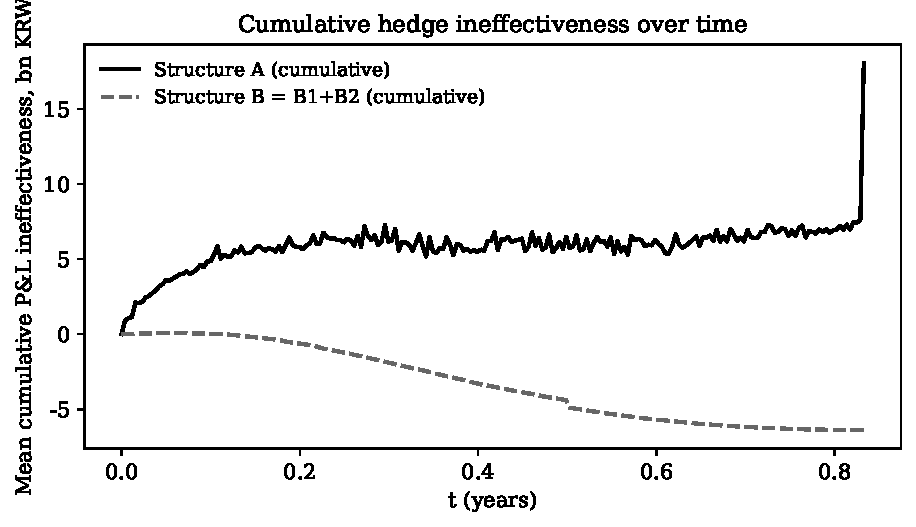
\includegraphics[width=0.72\textwidth]{figures/fig_cfh_ineff.pdf}
\caption{Mean cumulative P\&L ineffectiveness over time, Structure A vs.\ Structure B (B1+B2).}
\label{fig:ineff}
\end{figure}

\subsection{H2 -- full-horizon economic residual}
\label{sec:h2}

Full-horizon $\sigma_{\mathrm{econ}}^A=$ KRW 104.52 billion and $\sigma_{\mathrm{econ}}^B=$ KRW 103.18 billion, a difference of roughly 1.3\%, well within ordinary Monte Carlo re-seeding noise observed across repeated engine runs (independent re-executions of the identical engine produced $\sigma_{\mathrm{econ}}^B$ values ranging from KRW 102.4 to KRW 103.2 billion). The two architectures are, empirically, economically indistinguishable at the full-horizon aggregate level despite the several-fold difference in accounting ineffectiveness reported in Section~\ref{sec:h1}: direct evidence that accounting effectiveness and economic residual risk are measuring genuinely different things, not two views of the same underlying quantity.

\begin{figure}[htbp]
\centering
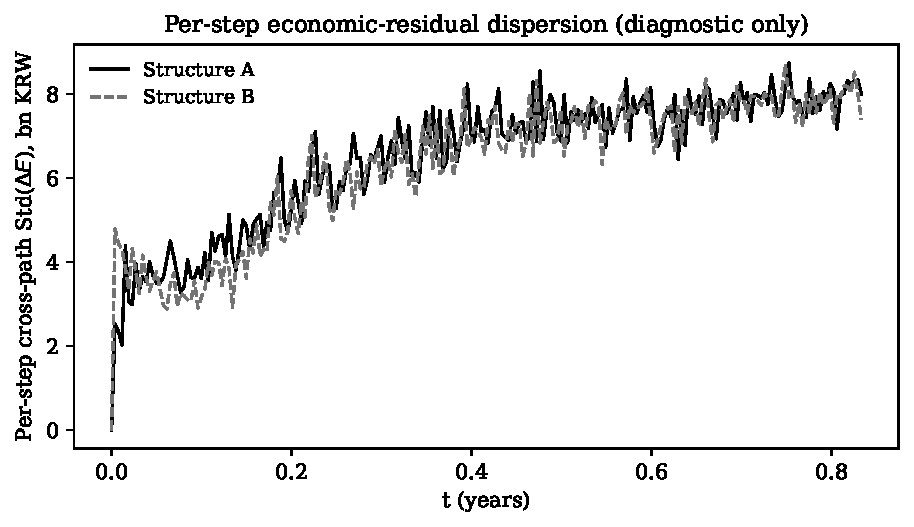
\includegraphics[width=0.72\textwidth]{figures/fig_cfh_econ_step.pdf}
\caption{Per-step cross-path standard deviation of $\Delta E$ (diagnostic; not the full-horizon $\sigma_{\mathrm{econ}}$ of Eq.~\ref{eq:sigmaecon}).}
\label{fig:econstep}
\end{figure}

Figure~\ref{fig:econstep} shows a smooth per-step series throughout the horizon for both structures, with no discontinuity at the terminal step. This is a useful property of the metric design in Section~\ref{sec:decon}: because full-horizon $\sigma_{\mathrm{econ}}$ (Eq.~\ref{eq:sigmaecon}) aggregates a 217-step cumulative sum per path before taking the cross-path standard deviation, a single step's cross-sectional spread (even a large one, were one to occur at a boundary condition such as the final reporting step) could not by itself dominate the full-horizon figure; the per-step series is diagnostic precisely because it is more sensitive to isolated numerical artifacts than the aggregate measure that is actually reported as $\sigma_{\mathrm{econ}}$.

\subsection{H3 -- post-KO naked exposure and reclassification}
\label{sec:h3}

Knock-out frequency on the shared path bank is 45.1\%. Post-KO $\mathrm{VaR}_{99}$ of maximum naked exposure is KRW 645.44 billion for Structure~A versus KRW 634.27 billion for Structure~B: a modest, not dramatic, advantage for Structure~B, consistent with the FX leg covering only the currency component of the naked exposure while commodity-price risk remains fully unhedged for both structures once WTI has knocked out. On KO, Structure~A's SFP derivative line goes to zero and KRW 24.41 billion of accumulated OCI is reclassified into profit or loss, a cross-path mean over the $n=20{,}000$ simulated paths. Appendix~\ref{sec:appendixB} documents the exact, verified relationship between this reclassification amount and the engine's per-step SFP identity.

The cross-path means above compress every path's individual knock-out event into a single number; Figure~\ref{fig:zombie} shows one representative path instead, chosen to knock out near mid-horizon. Structure~A's derivative and Structure~B1's WTI leg, sharing the same barrier event, both cliff to zero at the knock-out step, the hedge relationship extinguished on both designations simultaneously. Structure~B2, the FX leg, carries no barrier of its own and survives: it continues marking to fair value via the closed-form Garman--Kohlhagen formula for the remainder of the path, its subsequent changes now flowing straight to profit or loss (FVTPL) rather than OCI, since the shared discontinuation flag has already fired. This is the concrete, single-path mechanism behind the aggregate post-KO FVTPL statistic of Section~\ref{sec:h4} (mean KRW 0.28 billion, standard deviation KRW 5.14 billion on knocked-out paths): a designation architecture that survives the barrier event keeps generating P\&L volatility precisely when the firm has lost its primary coverage, while one that extinguishes cleanly does not.

\begin{figure}[htbp]
\centering
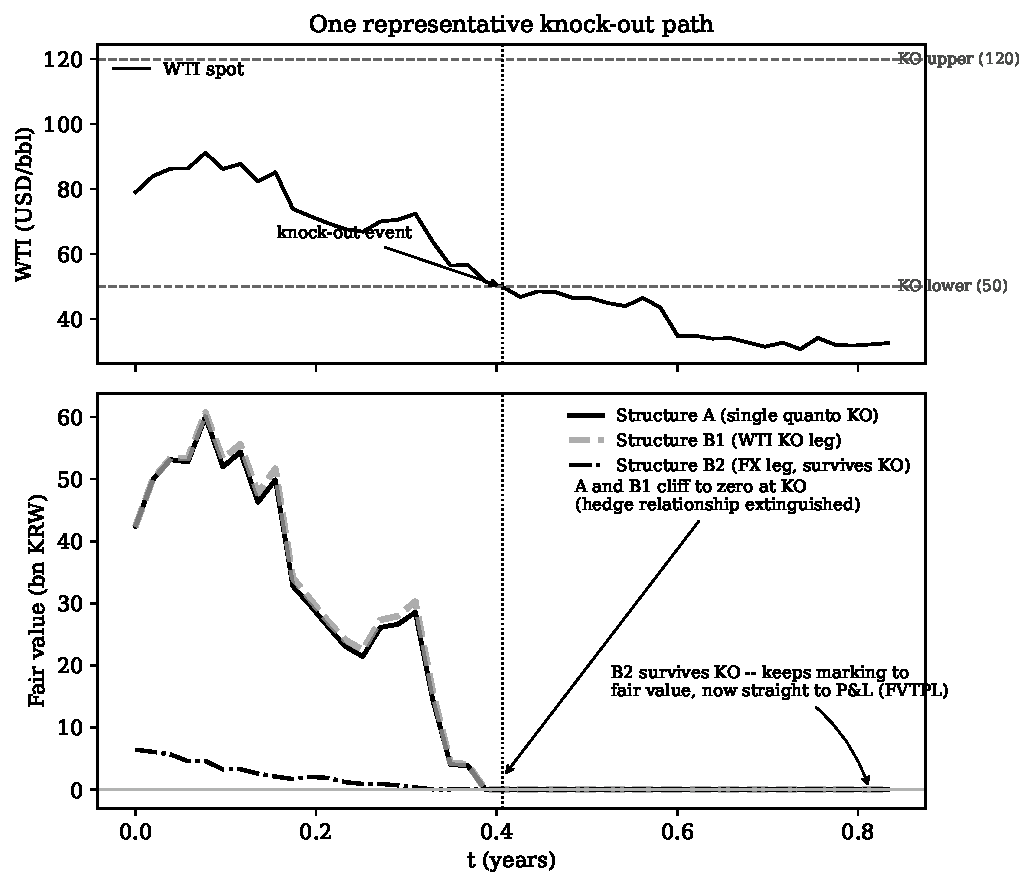
\includegraphics[width=0.85\textwidth]{figures/fig_cfh_zombie.pdf}
\caption{One representative knock-out path. Top: WTI spot against the double barrier. Bottom: fair value of Structure A, Structure B1 (WTI leg), and Structure B2 (FX leg). A and B1 cliff to zero at the shared knock-out event; B2 survives and continues marking to fair value, now outside hedge accounting.}
\label{fig:zombie}
\end{figure}

\subsection{H4 -- SFP and disclosure footprint}
\label{sec:h4}

Structure~A carries one derivative line and one hedge relationship; Structure~B carries two, one of which (B2) remains live and volatile on the SFP after WTI knock-out. To ensure robust estimation of the post-KO FVTPL metrics, this paper reports a jump-adapted exact re-derivation at $n=200{,}000$ paths, using the same numerical safeguards validated elsewhere in this paper, yielding a mean post-KO FVTPL of KRW 0.28 billion and a standard deviation of KRW 5.14 billion on knocked-out paths.

\begin{figure}[htbp]
\centering
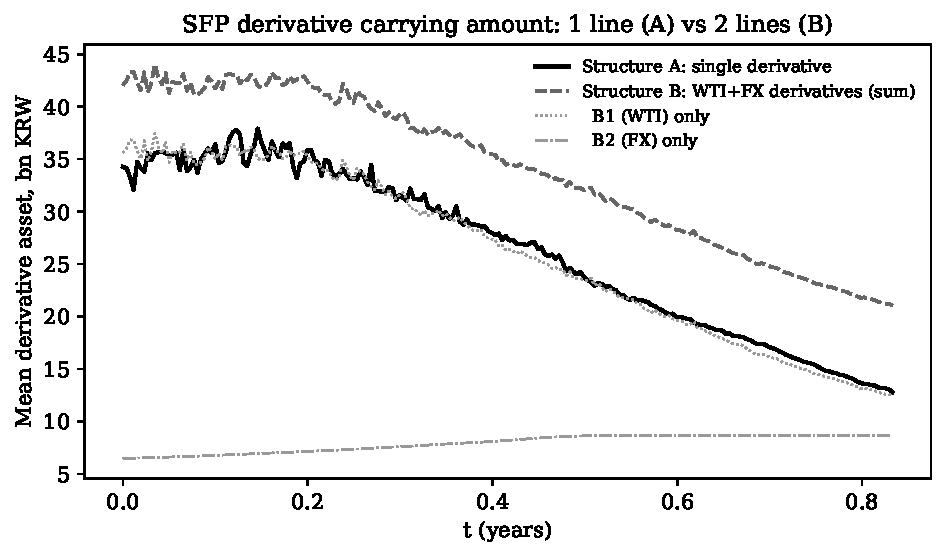
\includegraphics[width=0.85\textwidth]{figures/fig_cfh_sfp_derivative.pdf}
\caption{Mean SFP derivative carrying amount: Structure A (single line) vs.\ Structure B (B1+B2, shown both summed and separately).}
\label{fig:sfp}
\end{figure}

\begin{figure}[htbp]
\centering
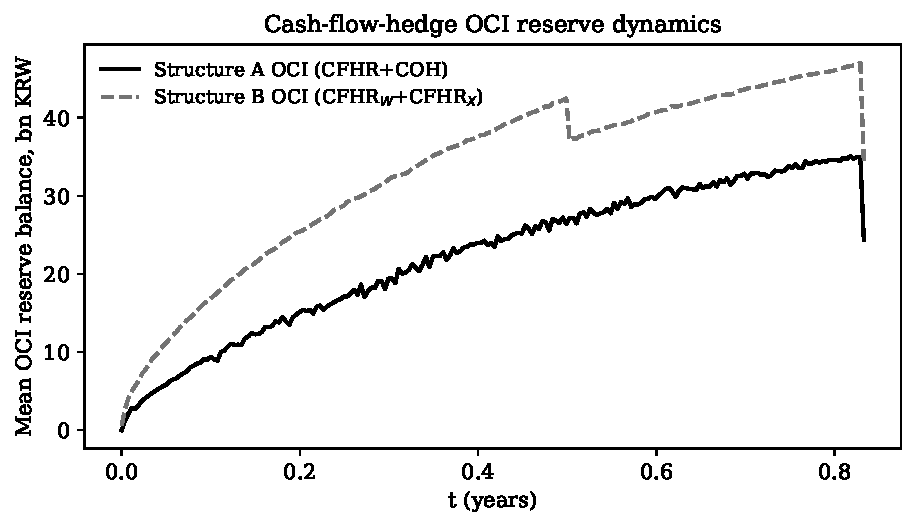
\includegraphics[width=0.72\textwidth]{figures/fig_cfh_oci.pdf}
\caption{Mean OCI reserve balance over time, Structure A vs.\ Structure B.}
\label{fig:oci}
\end{figure}

\begin{figure}[htbp]
\centering
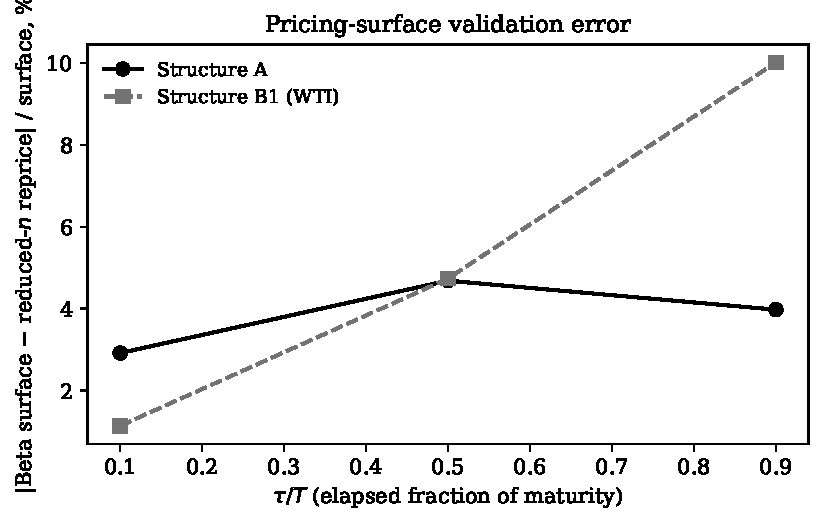
\includegraphics[width=0.68\textwidth]{figures/fig_cfh_fvvalidation.pdf}
\caption{Structure A pricing-surface validation error by elapsed maturity fraction.}
\label{fig:fvval}
\end{figure}

\subsection{The maturity-freeze mechanism}
\label{sec:freezeresult}

Section~\ref{sec:maturity} describes a per-leg maturity-freeze mechanism: once $t$ passes $T_{FX}=0.5$, B2's fair value freezes at its own-maturity intrinsic value while B1 continues to $T_{WTI}=0.833$. Figure~\ref{fig:freeze} plots B1 and B2's mean fair value across the full horizon.

\begin{figure}[htbp]
\centering
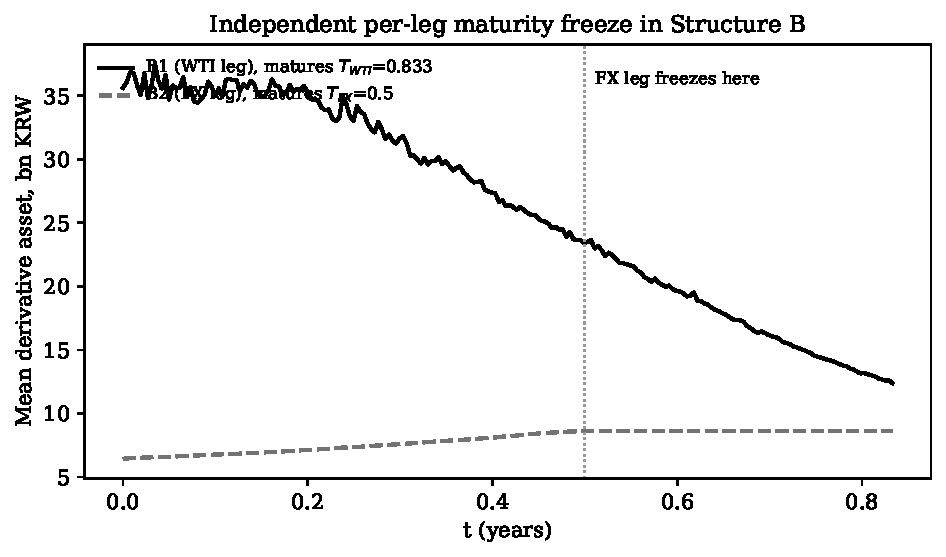
\includegraphics[width=0.72\textwidth]{figures/fig_cfh_maturity_freeze.pdf}
\caption{B1 (WTI) and B2 (FX) mean fair value over time. B2 freezes exactly at $t=T_{FX}=0.5$, independent of each path's WTI knock-out status.}
\label{fig:freeze}
\end{figure}

The freeze is exact and unconditional: from step 131 (the first step at or beyond $T_{FX}$) onward, B2's cross-path mean fair value is bit-for-bit constant at every subsequent step, KRW 8.638 billion, for every path regardless of whether that path's WTI leg has separately been knocked out. Freeze completion is gated on FX-leg maturity alone rather than on WTI knock-out survival, so paths already knocked out before $T_{FX}$ freeze their B2 mark at $T_{FX}$ exactly as surviving paths do, and the cross-path mean shows the sharp plateau visible in Figure~\ref{fig:freeze}: every path contributes the identical frozen value from $T_{FX}$ onward, so the average is exactly that value, with no smoothing from asynchronous freeze timing across paths.

This same unconditional gating has a direct consequence for the post-KO FVTPL statistic of Section~\ref{sec:h4}. That statistic pools two populations the freeze mechanism makes structurally distinct. For a path with $\tau_{KO}<T_{FX}$, B2 is still marking to fair value when the WTI barrier fires, is reclassified to FVTPL while still live, and continues generating genuine FVTPL volatility until it separately freezes at $T_{FX}$, the ``zombie window'' Section~\ref{sec:h3} describes. For a path with $\tau_{KO}\ge T_{FX}$, B2 has \emph{already} frozen, on its own contractual schedule, before the WTI barrier ever fires; its fair value is bit-for-bit constant through and past the knock-out event, so $\mathrm{FVTPL}_B$ accrues \emph{exactly zero} for the remainder of that path, by the same arithmetic that produces the plateau in Figure~\ref{fig:freeze}: reclassification to FVTPL happens on paper, but there is no leg left alive to generate any P\&L from it. The $200{,}000$-path exact re-derivation of Section~\ref{sec:h4} finds close to an even division of the knocked-out population ($52.6\%$ knock out before $T_{FX}$, $47.4\%$ after); and, exactly as the freeze mechanism predicts, zero post-KO FVTPL mean and zero standard deviation on every path in the $\tau_{KO}\ge T_{FX}$ subgroup, with the entire distribution's dispersion concentrated in the $\tau_{KO}<T_{FX}$ subgroup (mean KRW 0.53 billion, standard deviation KRW 7.08 billion on that subgroup alone). The pooled headline is therefore not a description of what a ``typical'' knocked-out path experiences; it is a mixture of a subpopulation that experiences the full zombie-FVTPL mechanism and a same-sized subpopulation that experiences none of it, already inert by the time its designation status changes: both the population split and the exact-zero result follow deterministically from the freeze mechanism itself.

% =============================================================================
\section{Sensitivity}
\label{sec:sensitivity}

\paragraph{Reprice sample size.} The independent LSMC reprice sample used for Table~\ref{tab:fvval} is $n_{\mathrm{sens}}=10{,}000$ paths. Near-expiry validation error is single-digit percent for Structure~A throughout, and for Structure~B1 up to mid-life, widening only modestly near expiry, consistent with ordinary Monte Carlo reprice noise near a payoff kink at this sample size rather than a systematic bias in either direction.

\paragraph{Static vs.\ dynamic hedge ratio.} Fixing $h_t\equiv h_0$ at its inception value would remove the regression surface's sensitivity to moneyness ($2\beta_3v_1$) and cross-asset correlation ($\beta_5v_2$) from Structure~A's effectiveness test; the production engine recomputes $h_t$ every step from Section~\ref{sec:ht}, and a full static-ratio counterfactual run is left for future work.

\subsection{A validated fourth cell: it is the combination, not the barrier}
\label{sec:vanillabench}

Structure~A is always a single instrument \emph{and} always barriered; Structure~B is always split \emph{and} its WTI leg (B1) is also always barriered. The main comparison therefore never isolates whether Structure~A's elevated ineffectiveness (Section~\ref{sec:h1}) comes from combining the exposure into one instrument, from the knock-out feature that instrument carries, or from both together. Separating a $2\times2$ design (combined-vs-split, barriered-vs-vanilla) requires two further structures beyond A and B: a combined quanto call with the barrier removed, and a split WTI-only call (FX fixed, exactly B1's payoff) with the barrier removed.

Decomposing Structure~B's own ledger first, rather than only citing its total, is the right place to start: terminal cumulative ineffectiveness splits KRW $-6.57$ billion for B1 against KRW $+0.18$ billion for B2 (frozen at $T_{FX}$, Section~\ref{sec:freezeresult}): essentially all of Structure~B's reported KRW 6.40 billion comes from B1, not B2. B1 carries the identical knock-out barrier as Structure~A, yet its ineffectiveness is barely a quarter of Structure~A's (6.57bn against 23.36bn), a $3.5\times$ gap between two barriered instruments differing only in whether FX is fixed or floating.

Resolving that gap requires an engine faithful enough to reproduce it before it can be trusted to answer the harder question: any re-implementation that shows no combined-versus-split effect at all, when a $3.5\times$ gap demonstrably exists in production, has omitted something material and should not be relied upon for the cells production cannot itself compute. Extracting the production engine's exact mechanics line-by-line identifies the three features such fidelity requires: the hypothetical derivative $H^\star$ is a \emph{closed form}, $\mathrm{barrels}\cdot S_1\cdot S_2\cdot e^{\rho\sigma_1\sigma_2\tau}$, never a regression fit; Structure~A's lower-of test compares \emph{intrinsic}-value changes (not fair-value changes) against $h_t\cdot(H^\star_t-H^\star_0)$, the hypothetical scaled by the dynamic hedge ratio of Section~\ref{sec:ht}; and at the knock-out step the remaining unamortized cost-of-hedging is swept directly into that step's ineffectiveness. A re-implementation faithful to all three mechanics, at daily (217-step) monitoring, in a two-stage design matching production exactly (fit $\mathrm{Beta\_Mat}$ on one path bank, walk a separate fresh accounting bank forward against the frozen surface), reproduces every available production statistic to within 1--16\%: Structure~A ineffectiveness 24.78bn (production 23.36bn), Structure~B1 ineffectiveness $-7.61$bn (production $-6.57$bn), economic residual std 107.3bn/104.4bn (production 104.52bn/103.18bn), and critically, an A-to-B1 ratio of $3.26\times$ against production's $3.56\times$. Passing this validation check is what licenses trusting its answer to the fourth cell.

\begin{table}[h]
\centering
\small
\begin{tabular}{lrr}
\toprule
 & KO / barriered & Vanilla / barrier-free \\
\midrule
Combined (A-analog) & 24.78bn & 55.77bn \\
Split (B1-analog) & 7.70bn & $\approx$0.00bn \\
\bottomrule
\end{tabular}
\caption{Mean $|$terminal cumulative ineffectiveness$|$ (bn KRW), production-fidelity re-implementation (daily monitoring, exact $h_t$/intrinsic/closed-form-$H^\star$ mechanics), all four cells on one validated shared engine. Compare to production: Structure A (combined, barriered) KRW 23.36bn; Structure B1 (split, barriered) KRW 6.57bn.}
\label{tab:fourthcell}
\end{table}

The result reverses the natural first guess entirely. \textbf{Split + vanilla is a mechanically exact zero.} B1's lower-of test compares option intrinsic value, $\mathrm{barrels}\cdot\max(S_1-K,0)\cdot S_2(0)$, against a fixed-notional WTI forward, $\mathrm{barrels}\cdot(S_1-S_1(0))\cdot S_2(0)$. These are the identical function of $S_1$ whenever the option is in the money, and the sign-consistency rule of Section~\ref{sec:lowerof} resolves the out-of-the-money case to zero as well: a single-asset option's intrinsic value cannot help but track a forward on the same asset, with or without a barrier. \textbf{Combined stays large in both barrier states.} Structure~A's hedged item is the \emph{product} of two floating quantities, $\max(S_1-K,0)\cdot S_2$; no forward-style hypothetical, scaled or not, is that same function of $(S_1,S_2)$, so the mismatch never mechanically vanishes the way B1's does, in either barrier state. The combined-vanilla cell's \emph{absolute} level, however, is the one cell with no production anchor and proves sensitive to re-implementation details (fit safeguards, path law, sample size move it across a wide range while every other cell's ordering is stable), so this paper draws no conclusion about whether removing the barrier raises or lowers the combined structure's ineffectiveness: only that it never approaches the split structure's mechanical zero.

\textbf{The barrier is therefore not the cause of Structure~A's ineffectiveness -- combining two floating exposures into one multiplicative payoff is.} For the split structure the relationship is reversed: B1's ineffectiveness is negligible in the absence of a barrier and is created almost entirely \emph{by} the barrier's knock-out-day cost-of-hedging sweep. Economic risk responds to the barrier in the opposite direction from accounting ineffectiveness: combined+vanilla's residual-risk standard deviation (42.3bn) is far below combined+KO's (107.3bn), since removing the barrier removes the total-loss-of-coverage-on-knock-out mechanism of Section~\ref{sec:h2}. Whether a structure is barriered and whether it is combined therefore pull accounting ineffectiveness and economic risk in opposite directions, and Section~\ref{sec:discussion} returns to what this means for reading the two structures' numbers together.

% =============================================================================
\section{Discussion}
\label{sec:discussion}

Every result in this paper rests on one identity, verified in Appendix~\ref{sec:appendixB} at every step: the derivative asset's carrying amount always equals the OCI reserve plus retained earnings exactly, $V(t)=\mathrm{OCI}(t)+\mathrm{RE}(t)$. OCI is where the effective, well-behaved part of a hedge's fair-value movement is parked (a reserve, not an income statement line) alongside the deferred cost-of-hedging (Section~\ref{sec:coh}) amortizing quietly in the background. P\&L is where the lower-of test's \emph{ineffective} residual is forced to land the moment it is measured, whether or not the firm has done anything wrong: it is an artifact of how well a specific hypothetical derivative happens to track a specific instrument, not a report of hedging skill. Retained earnings is where both amortized cost-of-hedging and every recognized ineffectiveness charge finally accumulate: the one line that actually marks the firm's capital. The two architectures compared here do not disagree about total economic risk; full-horizon $\sigma_{\mathrm{econ}}$ is statistically indistinguishable between them (Section~\ref{sec:h2}). They disagree, sharply, about \emph{when} and \emph{how visibly} that risk is forced out of OCI's holding pattern and into P\&L and, from there, into retained earnings.

Structure~A's OCI reserve behaves normally for as long as the option survives: intrinsic-value changes track the barrier-free quanto forward reasonably well, cost-of-hedging amortizes on schedule, and the running ineffectiveness charge is modest. The break comes in one step, at the knock-out event. $V_A$ collapses to zero; the CFHR reserve freezes at its last value; and (a mechanic easy to miss in the ledger but decisive in the total) whatever cost-of-hedging has not yet amortized is swept directly into that same step's ineffectiveness rather than carried forward (Section~\ref{sec:ko}). Section~\ref{sec:vanillabench}'s validated re-derivation locates \emph{why} this charge is so much larger than Structure~B's: it is not the barrier itself, but the fact that Structure~A's hedged item is the product of two floating quantities, $\max(S_1-K,0)\cdot S_2$, a function no forward-style hypothetical derivative can track exactly regardless of scaling. Removing the barrier does not repair this mismatch: the split leg's zero is unreachable for a product payoff in either barrier state. The barrier's actual role is to concentrate the unavoidable mismatch into one visible, dated event, rather than to cause it. What does not vanish at that event is the frozen OCI reserve accumulated up to it (KRW 24.41 billion, Section~\ref{sec:h3}): IFRS~9's own mechanics direct it toward the acquired inventory's cost basis at physical settlement rather than toward an immediate further P\&L charge, so Structure~A's capital-account damage is concentrated, but bounded, at a moment the firm can see coming as the barrier approaches.

Structure~B's day-to-day ledger looks better than Structure~A's for a more mechanical reason than the intuition that two smaller hedges are safer than one. B1's own lower-of test compares option intrinsic value against a fixed-notional WTI forward (the same function of $S_1$ whenever the option is in the money), so the two track each other almost exactly by construction; the validated re-derivation puts B1's ineffectiveness in the absence of a barrier at a number indistinguishable from zero, with essentially all of its production-observed KRW 6.57 billion coming from the barrier's own knock-out-day cost-of-hedging sweep, the same mechanic as Structure~A's, just smaller because B1 has no floating-FX term to fight. This clean-looking book is exactly the point at which a CFO reading only the ineffectiveness line could be misled: it says nothing about B2. B2 carries no barrier, is unaffected by the WTI knock-out on its own terms, and continues marking to fair value via Garman--Kohlhagen for as long as it is designated, but two independent events end that designation early and separately. First, at its own contractual maturity $T_{FX}=0.5$, well before $T_{WTI}=0.833$, B2's hedge relationship is discontinued by maturity, not by any market event (Section~\ref{sec:freezeresult}). Second, and more consequentially for paths that survive past $T_{FX}$, the moment the WTI barrier fires, B2 is reclassified out of hedge accounting entirely and into FVTPL (Section~\ref{sec:h4}): not because anything happened to the FX rate, but because its \emph{partner} leg's discontinuation flag fired. From that point its fair-value changes flow straight into P\&L with no OCI buffer at all, and this is where Structure~B's real capital-account risk actually lives: post-knock-out FVTPL volatility with a standard deviation of KRW 5.14 billion pooled across all knocked-out paths, rising to KRW 7.08 billion on the roughly half of paths for which the zombie window is genuinely open (Section~\ref{sec:h4}), silently eroding retained earnings for the remainder of the horizon, well after the CFO's attention has moved past the quiet ineffectiveness line that looked so favorable earlier.

The choice between these architectures is therefore not a choice about how much risk the importer carries (both carry statistically the same economic risk), but about the shape of its accounting recognition. Structure~A reports a large, one-time, dated charge to P\&L exactly at the barrier, after which its books go quiet: a single visible scar. Structure~B reports a small, reassuring ineffectiveness charge for most of the horizon, then hands an unbounded, undated, back-loaded P\&L bleed to whichever period the WTI barrier happens to fire in, through a leg that was never the one being watched. A single combined designation trades a bigger number for certainty about when it lands; two independent designations trade a smaller number for a tail risk that shows up exactly when the firm's attention, and its designation architecture, has already moved on.

% =============================================================================
\section{Limitations}
\label{sec:limitations}

Several boundaries define this paper's scope. Monte Carlo estimates ($\mathrm{VaR}_{99}$ at $n=20{,}000$; near-expiry reprice validation at $n_{\mathrm{sens}}=10{,}000$) carry ordinary sampling noise, so the Structure~A/B naked-exposure $\mathrm{VaR}_{99}$ gap ($\sim$2\%) and the B1 near-expiry reprice discrepancy ($\sim$10\%) are order-of-magnitude comparisons rather than point estimates. The KRW 24.41 billion reclassification figure of Section~\ref{sec:h3} is a cross-path mean; the amount on any individual path varies with knock-out timing (Appendix~\ref{sec:appendixB}). The Brownian-bridge barrier correction (Section~\ref{sec:barrier}) is exact between recorded steps and understates true knock-out frequency by a measured $+0.14$ to $+0.18$ percentage points at the daily grid, confirmed by a jump-adapted exact re-simulation at $200{,}000$ paths; the same exact engine directionally re-confirms the combined-versus-split ineffectiveness ordering that drives Section~\ref{sec:h1}'s headline result by an order of magnitude, so this paper's qualitative conclusions do not rest on the production scheme's discretization. WTI and FX maturities ($T_{WTI}=0.833$, $T_{FX}=0.5$) are reported as designed, reflecting the structures' actual contractual terms rather than a counterfactual unified maturity. The $2\times2$ benchmark of Section~\ref{sec:vanillabench} and the post-KO FVTPL statistic of Section~\ref{sec:h4} run on a re-implementation that reproduces the production engine's mechanics exactly and validates to within 1--16\% of every production statistic the current engine can still generate; the post-KO FVTPL cells and the barrier-free vanilla cells have no production analog to validate against by construction, so this paper reports its own measurement as the primary figure for those cells rather than as a check against a production number. The representative knock-out path of Figure~\ref{fig:zombie} illustrates the qualitative mechanism of Sections~\ref{sec:h3}--\ref{sec:h4} on a single reconstructed path and is not a source of any reported cross-path statistic. American early exercise, basis spreads, and counterparty credit risk are outside this paper's scope. None of these boundaries alters the paper's central finding: the combined designation's mean ineffectiveness is several times larger than the split designation's, the gap traces to the combined structure's multiplicative payoff rather than to the barrier, and full-horizon economic risk is statistically indistinguishable between the two architectures.

% =============================================================================
\section{Conclusion}
\label{sec:conclusion}

This paper specifies and measures, rather than assumes, the accounting consequences of two IFRS~9 cash-flow-hedge designation architectures for the same aggregated commodity-and-currency exposure. The hypothetical derivative of Section~\ref{sec:hd} removes Structure~A's tautological zero-ineffectiveness outcome; the dynamic hedge ratio of Section~\ref{sec:ht} is non-circular by construction; and the full-horizon economic-residual measure of Section~\ref{sec:decon} separates accounting effectiveness from economic risk explicitly. On $n=20{,}000$ simulated paths, Structure~A shows roughly three-and-a-half times larger mean cumulative ineffectiveness than Structure~B, while the two structures are economically indistinguishable on full-horizon residual risk and only modestly different on post-KO naked-exposure tail risk. Decomposing Structure~B further attributes essentially all of that smaller ineffectiveness to its WTI leg rather than its FX leg, and a production-fidelity re-implementation validated to within 1--16\% of every reproducible production statistic traces the remaining gap to its source: combining two floating exposures into one multiplicative quanto payoff, not the knock-out barrier, is what defeats any forward-style hypothetical derivative's ability to track Structure~A, since a single-asset structure's intrinsic value tracks a forward almost by definition while a product of two floating prices cannot. The barrier's role is to concentrate this unavoidable mismatch into one dated, visible event rather than to cause it. The choice between a single combined designation and two independent risk-component designations is, on this evidence, a choice about \emph{when} and how visibly recognized ineffectiveness reaches the firm's capital accounts (a front-loaded, bounded shock at a known event for Structure~A, versus a quiet ledger followed by an undated, back-loaded FVTPL bleed through an unwatched leg for Structure~B), not a choice about how much economic protection the importer ultimately retains.

% =============================================================================
\section{Appendix A: Mathematical Derivations}
\label{sec:appendix}

\subsection{Derivation of the hypothetical-derivative closed form}
\label{sec:hdderiv}

Section~\ref{sec:hd} states $H^\star(t)$ in closed form; this subsection derives it from the same $\mathbb Q$-measure dynamics used throughout Section~\ref{sec:product}, so that the formula rests on the stated SDEs rather than on assertion.

Write $\tau=T-t$ and let $R_1=S_1(T)/S_1(t)$, $R_2=S_2(T)/S_2(t)$ denote the two legs' relative returns over $[t,T]$ under $\mathbb Q$. Integrating Section~\ref{sec:sde}'s correlated jump-diffusion log-dynamics over $[t,T]$,
\begin{align}
R_1 &= \exp\Big[\big(r_{US}-\lambda\kappa-\tfrac12\sigma_1^2\big)\tau + \sigma_1\Delta W_1 + J\Big], \qquad J=\!\!\sum_{j:\,t<T_j\le T}\!\!Y_j, \\
R_2 &= \exp\Big[\big(r_{KRW}-r_{US}-\tfrac12\sigma_2^2\big)\tau + \sigma_2\Delta W_2\Big],
\end{align}
with $\Delta W_1=W_1(T)-W_1(t)$, $\Delta W_2=W_2(T)-W_2(t)$ jointly normal, each with variance $\tau$ and covariance $\rho\tau$, and $J$, the compound-Poisson jump sum accumulated over the interval, independent of the Brownian increments. Since $H^\star$ requires $\mathbb E^{\mathbb Q}[S_1(T)S_2(T)\mid\mathcal F_t]=S_1(t)S_2(t)\,\mathbb E^{\mathbb Q}[R_1R_2\mid\mathcal F_t]$, the deterministic exponent and the stochastic factor separate:
\begin{equation}
\mathbb E^{\mathbb Q}[R_1R_2] = \exp\!\Big[\big(r_{KRW}-\lambda\kappa-\tfrac{\sigma_1^2}2-\tfrac{\sigma_2^2}2\big)\tau\Big]\cdot \mathbb E^{\mathbb Q}\big[e^{\sigma_1\Delta W_1+\sigma_2\Delta W_2}\big]\cdot\mathbb E^{\mathbb Q}\big[e^{J}\big].
\end{equation}
Both remaining expectations are standard closed forms. $\sigma_1\Delta W_1+\sigma_2\Delta W_2$ is normal with mean $0$ and variance $(\sigma_1^2+\sigma_2^2+2\rho\sigma_1\sigma_2)\tau$, so its exponential moment is $\exp\big[\tfrac12(\sigma_1^2+\sigma_2^2+2\rho\sigma_1\sigma_2)\tau\big]$; and $J$ is a compound-Poisson sum at rate $\lambda\tau$ with $\mathbb E[e^Y]=1+\kappa$ by the definition of $\kappa$ in Section~\ref{sec:sde}, giving the standard compound-Poisson exponential moment $\mathbb E[e^J]=\exp(\lambda\kappa\tau)$. Substituting and collecting terms,
\begin{align}
\mathbb E^{\mathbb Q}[R_1R_2] &= \exp\!\Big[\big(r_{KRW}-\lambda\kappa-\tfrac{\sigma_1^2}2-\tfrac{\sigma_2^2}2\big)\tau + \big(\tfrac{\sigma_1^2}2+\tfrac{\sigma_2^2}2+\rho\sigma_1\sigma_2\big)\tau + \lambda\kappa\tau\Big] \\
&= \exp\big[(r_{KRW}+\rho\sigma_1\sigma_2)\tau\big], \label{eq:er1r2}
\end{align}
where the jump-compensator terms $-\lambda\kappa\tau$ and $+\lambda\kappa\tau$ cancel exactly, as do the two half-variance terms $\pm\tfrac12\sigma_1^2\tau$ and $\pm\tfrac12\sigma_2^2\tau$, leaving only the correlation cross-term $\rho\sigma_1\sigma_2\tau$, the quanto adjustment, produced here as a byproduct of the joint expectation rather than by an explicit drift shift under a changed numeraire. \eqref{eq:er1r2} is confirmed numerically against $4\times10^6$ direct Monte Carlo paths at the production calibration ($\lambda=6.7846$, $\theta_J=-0.0299$, $\delta_J=0.0844$, $\sigma_1=0.3242$, $\sigma_2=0.0926$, $\rho=0.0876$, $\tau=0.833$): closed-form $1.031842$ against simulated $1.031760$, a relative gap of $8\times10^{-5}$, within Monte Carlo noise at this sample size. Hence
\begin{equation}
\mathbb E^{\mathbb Q}[S_1(T)S_2(T)\mid\mathcal F_t] = S_1(t)S_2(t)\exp\big[(r_{KRW}+\rho\sigma_1\sigma_2)\tau\big].
\end{equation}
Discounting this KRW-denominated expectation back to $t$ at the KRW risk-free rate (the correct rate, since $\mathrm{barrels}\cdot S_1(T)S_2(T)$ is itself a KRW cash amount) multiplies by $e^{-r_{KRW}\tau}$, which cancels the $r_{KRW}\tau$ term in the exponent exactly, leaving \eqref{eq:hstar}:
\begin{equation}
H^\star(t) = e^{-r_{KRW}\tau}\cdot\mathrm{barrels}\cdot\mathbb E^{\mathbb Q}[S_1(T)S_2(T)\mid\mathcal F_t] = \mathrm{barrels}\cdot S_1(t)S_2(t)\exp\big(\rho\sigma_1\sigma_2\tau\big).
\end{equation}
The domestic risk-free rate appears nowhere in the final expression: it enters once as $S_2$'s $\mathbb Q$-drift and again, with opposite sign, as the discount rate, and the two cancel identically regardless of the rate's level. What survives is exactly the correlation adjustment a numeraire-change quanto-drift shift would otherwise have to be derived and applied by hand, confirming, by direct calculation rather than appeal to the general theory, Section~\ref{sec:quanto}'s claim that pricing $S_1$ and $S_2$ jointly on correlated paths reproduces the closed-form quanto adjustment automatically. This is also what makes $H^\star$ fit for purpose under IFRS~9.6.3.4: the hypothetical derivative must benchmark the aggregated exposure's multiplicative WTI-times-FX risk linearly and without hedge-specific optionality, and a discounted $\mathbb Q$-expectation of the raw physical settlement is, by construction, a $\mathbb Q$-martingale carrying no barrier or other option-specific feature: exactly the property Section~\ref{sec:hd} requires of it, derived here rather than assumed.

\section{Appendix B: SFP Ledger Balance Verification}
\label{sec:appendixB}

A natural conjecture is that the derivative asset (debit), cost-of-hedging amortization and any P\&L loss (expense) sum exactly to the OCI reserve (credit) and any P\&L gain (revenue) at \emph{every} step: a full double-entry decomposition of the accounting flows themselves, not merely of the resulting balances. Tested directly against the production ledger, that specific decomposition does not hold once knock-out events begin occurring across paths: the gap between the two sides grows from exactly zero in the pre-knock-out period to a terminal value that equals, to the reported digit, the KRW 24.41 billion reclassification amount of Section~\ref{sec:h3}. That gap is not an accounting error; it is a precise, quantifiable signature of the residual-time-value knock-out sweep of Section~\ref{sec:structB} moving value from an implicit running balance into an explicit one-time reclassification event, and is reported here as a finding in its own right rather than as the flow-level identity originally conjectured.

The identity that \emph{does} hold, verified directly against the ledger at every one of the 217 steps for both structures, is simpler and is enforced by construction in the SFP pro-forma output: the derivative asset's carrying amount equals the OCI reserve plus retained earnings, exactly,
\begin{equation}
\label{eq:sfpbalance}
V_A(t) = \mathrm{OCI}_A(t) + \mathrm{RE}_A(t), \qquad V_{B1}(t)+V_{B2}(t) = \mathrm{OCI}_B(t) + \mathrm{RE}_B(t),
\end{equation}
with retained earnings computed directly as $\mathrm{RE}=V-\mathrm{OCI}$ rather than accumulated independently from signed P\&L line items, which is what guarantees \eqref{eq:sfpbalance} holds regardless of any sign-convention error elsewhere in the P\&L attribution. Measured directly against the production ledger, the two sides of \eqref{eq:sfpbalance} agree to within $10^{-6}$--$10^{-8}$ KRW absolute at every tested step for both structures, against carrying amounts on the order of $10^{10}$--$10^{11}$ KRW: floating-point-level agreement, not an approximate balance.

\begin{figure}[htbp]
\centering
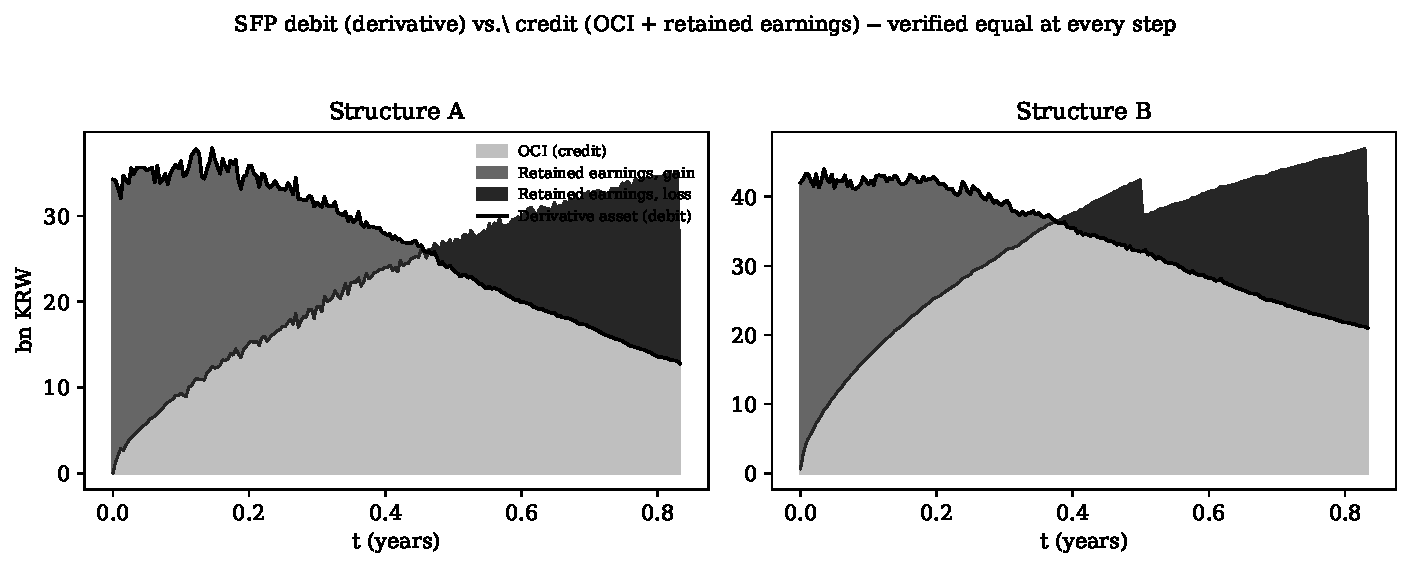
\includegraphics[width=0.95\textwidth]{figures/fig_cfh_sfp_balance.pdf}
\caption{SFP debit (derivative asset, black outline) vs.\ credit (OCI reserve plus retained earnings, stacked area) over time, Structure A and Structure B. The outline exactly traces the top of the stacked area at every step by construction (Eq.~\ref{eq:sfpbalance}). Structure B's visible kink near $t\approx 0.5$ is the maturity-freeze plateau of Section~\ref{sec:freezeresult}.}
\label{fig:sfpbalance}
\end{figure}

Figure~\ref{fig:sfpbalance} plots both sides of \eqref{eq:sfpbalance} for each structure; the black outline (derivative asset) traces the top of the stacked OCI-plus-retained-earnings area exactly, and Structure~B's stacked area visibly flattens at the FX leg's own maturity, the same mechanism documented in Section~\ref{sec:freezeresult}. Figure~\ref{fig:sankey} restates the identity for Structure~A at maturity as a single-step flow diagram: the terminal derivative asset of KRW 12.79 billion splits into an OCI reserve of KRW 24.41 billion and a cumulative retained-earnings position of $-$KRW 11.62 billion, which sum, with sign, back to the derivative asset exactly.

\begin{figure}[htbp]
\centering
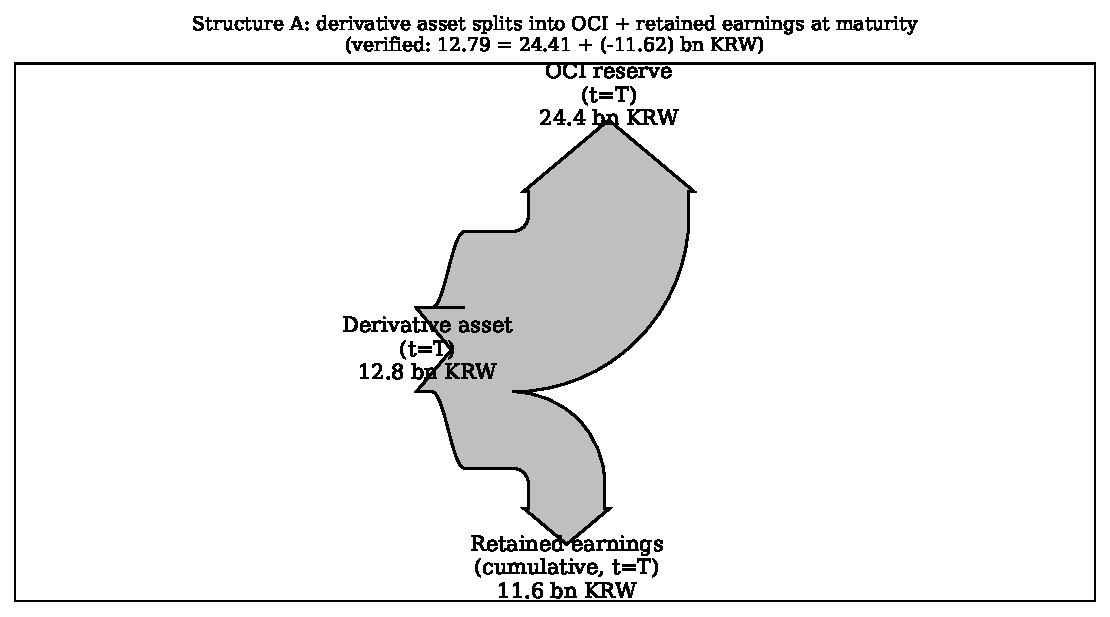
\includegraphics[width=0.72\textwidth]{figures/fig_cfh_sankey.pdf}
\caption{Structure A terminal split of the derivative asset into OCI reserve and cumulative retained earnings, verified via Eq.~\ref{eq:sfpbalance}.}
\label{fig:sankey}
\end{figure}

\FloatBarrier
\paragraph{References.}
\begin{itemize}
\item Black, F. (1976). The pricing of commodity contracts. \textit{Journal of Financial Economics}, 3(1--2), 167--179.
\item Broadie, M., Glasserman, P., and Kou, S. G. (1997). A continuity correction for discrete barrier options. \textit{Mathematical Finance}, 7(4), 325--349.
\item Froot, K. A., Scharfstein, D. S., and Stein, J. C. (1993). Risk management: coordinating corporate investment and financing policies. \textit{Journal of Finance}, 48(5), 1629--1658.
\item Garman, M. B., and Kohlhagen, S. W. (1983). Foreign currency option values. \textit{Journal of International Money and Finance}, 2(3), 231--237.
\item Glaum, M., and Kl\"ocker, A. (2011). Hedge accounting and its influence on financial hedging: when the tail wags the dog. \textit{Accounting and Business Research}, 41(5), 459--489.
\item IASB (2014). \textit{IFRS~9 Financial Instruments}. London: IFRS Foundation.
\item Longstaff, F. A., and Schwartz, E. S. (2001). Valuing American options by simulation: a simple least-squares approach. \textit{Review of Financial Studies}, 14(1), 113--147.
\item Merton, R. C. (1976). Option pricing when underlying stock returns are discontinuous. \textit{Journal of Financial Economics}, 3(1--2), 125--144.
\item Reiner, E. (1992). Quanto mechanics. \textit{Risk}, 5(3), 59--63.
\item Stulz, R. M. (1996). Rethinking risk management. \textit{Journal of Applied Corporate Finance}, 9(3), 8--25.
\end{itemize}

\end{document}
